%%% LaTeX Template: Two column assignment for BRSU
%%% Based on two column article from: http://www.howtotex.com/
%%% Preamble
\documentclass[	DIV=calc,%
				paper=a4,%
				fontsize=11pt,%
				twocolumn]{scrartcl}	 % KOMA-article class

\usepackage{lipsum}	% Package to create dummy text
\usepackage{blindtext}
\usepackage[english]{babel}	                          % English language/hyphenation
\usepackage[protrusion=true,expansion=true]{microtype} % Better typography
\usepackage{amsmath,amsfonts,amsthm}					 % Math packages
\usepackage[pdftex]{graphicx}	                          % Enable pdflatex
\usepackage[svgnames]{xcolor}	                          % Enabling colors by their 'svgnames'
\usepackage[hang, small,labelfont=bf,up,textfont=it,up]{caption} % Custom captions under/above floats
\usepackage{epstopdf}	 % Converts .eps to .pdf
\usepackage{subfig}	     % Subfigures
\usepackage{booktabs}	 % Nicer tables
\usepackage{fix-cm}       % Custom fontsizes
\usepackage{listings}
\usepackage{soul}
\usepackage{url}

%%% Custom sectioning (sectsty package)
\usepackage{sectsty}	 % Custom sectioning (see below)
\allsectionsfont{%% Change font of al section commands
	\usefont{OT1}{phv}{b}{n}%% bch-b-n: CharterBT-Bold font
	}

\sectionfont{%% Change font of \section command
	\usefont{OT1}{phv}{b}{n}%% bch-b-n: CharterBT-Bold font
	}


\definecolor{brsugrey}{rgb}{0.9, 0.9, 0.9}
\definecolor{brsublue}{rgb}{0, 0.594, 0.949}


\newcommand{\upperRomannumeral}[1]{\uppercase\expandafter{\romannumeral#1}}

%%% Headers and footers
\usepackage{fancyhdr} % Needed to define custom headers/footers
	\pagestyle{fancy} % Enabling the custom headers/footers
\usepackage{lastpage}	

% Header (empty)
\lhead{}
\chead{}
\rhead{}
% Footer (you may change this to your own needs)
\lfoot{\footnotesize 
\texttt{LAA} % Set to the course abbreviation 
\textbullet ~ Lang % Set to your name
\textbullet ~ Project Proposal } % Set the assignment number
\cfoot{}
\rfoot{\footnotesize page \thepage\ of \pageref{LastPage}}	% "Page 1 of 2"
\renewcommand{\headrulewidth}{0.0pt}
\renewcommand{\footrulewidth}{0.4pt}



%%% Creating an initial of the very first character of the content
\usepackage{lettrine}
\newcommand{\initial}[1]{%
     \lettrine[lines=3,lhang=0.3,nindent=0em]{
     				\color{brsublue}
     				{\textsf{#1}}}{}}

%%% Title, author and date metadata
\usepackage{titling}	% For custom titles

\newcommand{\HorRule}{\color{brsublue}% Creating a horizontal rule
					 \rule{\linewidth}{1pt}%
					 \color{black}
					 }

\pretitle{\vspace{-30pt} \begin{flushleft} \HorRule 
				\fontsize{25}{25} \usefont{OT1}{phv}{b}{n} \color{gray} \selectfont 
				}
\title{Learning and Adaptivity
\\ Assignment ~\upperRomannumeral{3} \\ - Project Proposal - }% Title of your article goes here
\posttitle{\par\end{flushleft}\vskip 0.5em}

\preauthor{\begin{flushleft}
\large \lineskip 0.25em \usefont{OT1}{phv}{b}{sl} \color{brsublue}}
\author{Bastian Lang~}	% Author name goes here
\postauthor{\footnotesize \usefont{OT1}{phv}{m}{sl} \color{Black} 
BRS University of Applied Sciences % Institution of author
\\email: bastian.lang@smail.inf.h-brs.de
\par\end{flushleft}\HorRule}

\date{\today} 

%%% Begin document
\begin{document}
\maketitle
\thispagestyle{fancy} % Enabling the custom headers/footers for the first page 
% The first character should be within \initial{}
\initial{T}\textbf{his course requires the students to work on a project were they will gain hands on experience with Machine Learning \& Adaptivity. The project should be manageable in 5 weeks. This proposal introduces a project about using machine learning techniques to learn a data-driven model of the Stella's velomobile.}


\section{Objective}
   
	\begin{figure}[h]
  		\centering
  		\caption{Stella's velomobiles.}
  		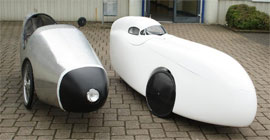
\includegraphics[width=0.4\textwidth]{./data/velomobile.jpg}
  		\label{fig:stella}
	\end{figure}   

	In the \textit{Stella Efficient Mobility} group of BRSU the focus lies on energy-efficient control and design of vehicles and the relationship between human and vehicle. 
	The goal is to use state-of-the-art machine learning solutions to solve traditional transportation problems\cite{stella}.
	Using techniques such as evolutionary algorithms to design controllers for the vehicles require simulated runs over test tracks.
	For this simulation a model of the vehicle is required.
	Due to the experimental design of the vehicles, a precise model is often times not known and models used usually only are approximations.
	Additionally if the used models are too complicated, the computation time gets high and simulation becomes slow.
	Poor approximations on the other hand may lead to problems when transferring solutions created through simulations to the real world.
	Artificial Neural Networks are capable of representing any dynamical system, so they are also capable of representing the model of a vehicle.
	The big advantage of ANNs is their low memory usage and their fast response.
	
	In this project I would like to create a data-driven vehicle model for Stella's white velomobile(see figure \ref{fig:stella}) by training an ANN using data obtained on test tracks.
	The exact method of training the ANN could be an evolutionary algorithm.
	
	Using the above methods to learn a vehicle model could lead to a vehicle model that is fast enough to be used within simulation and accurate enough to prevent from a huge performance loss in reality.
	
	If I would have more than five weeks I would apply the obtained model to an evolutionary algorithm to create autonomous energy efficient vehicle controllers for the velomobile.
	

\section{Data}

    
    In this project I am going to use data that I will collect by driving the velomobile on test tracks and recording necessary data.
    The data I am going to record is velocity, slope, motor commands, energy usage and travelled distance (by using gps and/or odometry).
    The final model shall be able to predict the energy usage and the resulting velocity in the next time step.
    Because I record all important data, the final data set will be labelled.



\section{Method}

	The model will be an Artificial Neural Network. 
	I have not entirely made up my mind about the exact type of ANN, but a Recurrent Neural Network seems to be a good choice.
	For training evolutionary algorithms such as \textit{Enforced SubPopulations} \cite{gomez2003active} or \textit{NEAT}\cite{stanley2002evolving} could be used.
	NEAT is currently one very famous technique for neuroevolution (over 1700 cites).
	Among others it has been applied in \cite{gaier2014evolving}.
	I am going to use Matlab and/or Python to do the implementation.

\section{Features}

	As mentioned above the data set will involve information about the velocity, slope, given motor command, gps coordinates and odometry data at sampled time steps.


\section{Milestones}

	\subsection{Week 1}
	The vehicles motor controller has to be adapted to collecting and recording data.
	This will be done within or even before week one.
	
	\subsection{Week 2}
	The remaining time of week one and week two will be needed for collecting data.
	
	\subsection{Week 3 - 4}
	The ANN and the learning technique have to be implemented and applied to the data.
	
	\subsection{Week 5}
	The actual performance of the model will be compared to the collected data and some easy model taken from \cite{gaier2014evolving}.
	
	\subsection{Presentation}
	The computational most intense part will be the training of the model. 
	Any live demo will probably not be of much value.
	So I plan to show graphs about the training progress, some figures demonstrating the whole learning process and some statistics comparing the performance of the learned model to the ground data and a simple model.
	

\bibliographystyle{plain}
\bibliography{./data/literature.bib}



\end{document}